\documentclass[docmute]{article}

% AMS packages for enhanced math typesetting and symbols:
\usepackage{amsmath}  % Provides enhanced math features like align, gather, etc.
\usepackage{amssymb}  % Provides additional math symbols
\usepackage{amsthm}   % Enables theorem-like environments

\usepackage{graphicx} % Provides commands for including and managing external graphics (e.g., figures, images)

% Package for customizing list environments:
\usepackage{enumitem} % Allows control over layout of lists (itemize, enumerate, etc.)

% Full-page layout package:
\usepackage{fullpage} % Uses more of the page area by reducing margins

% TikZ package for drawing graphics:
\usepackage{tikz}     % Used for creating high-quality diagrams and figures

% Microtype package for typographical enhancements:
\usepackage{microtype} % Improves justification, kerning, and overall appearance

% Package for typesetting polynomials:
\usepackage{polynom}  % Provides commands for polynomial long division and related tasks

% Package for controlling figure placement:
\usepackage{placeins} % Provides the \FloatBarrier command to control floating environments

% Forest package for drawing trees:
\usepackage{forest}   % Simplifies the creation of tree diagrams

% Package to allow one LaTeX file to input another:
\usepackage{docmute}  % Allows this file to be included in another document without reloading the preamble

% Load additional TikZ libraries:
\usetikzlibrary{trees} % Provides additional tree-specific commands for TikZ

% Define theorem-like environments using amsthm:
\newtheorem{corollary}{Corollary} % Defines a new "corollary" environment
\newtheorem{lemma}{Lemma}         % Defines a new "lemma" environment


% watermark.tex
\usepackage{everypage}  % For running code on every page
\usepackage{tikz}       % For drawing the watermark overlay
\usepackage{xcolor}     % For color options
\usepackage{graphicx}   % For including graphics

\AddEverypageHook{%
  \ifodd\value{page}
    % Do nothing on odd pages
  \else
    % On even pages, add the watermark image:
    \begin{tikzpicture}[remember picture, overlay]
      \node[rotate=0, opacity=0.1] at (current page.center) {%
        \includegraphics[width=0.6\paperwidth]{watermark.png}%
      };
    \end{tikzpicture}%
  \fi
}


\title{Partitions and Stirling Numbers}
\author{Tomasz Brengos \\  
Committers : Mykhailo Moroz}
\date{}

\begin{document}
\maketitle

\section{Set Partitions}  
\paragraph{Definition:}  
A set \( \{ A_1, A_2, \dots, A_k \} \) of subsets of \( N \) forms a \emph{partition of} the set \( N \) if:
\[
A_i \neq \emptyset, \quad A_i \cap A_j = \emptyset \text{ for } i \neq j, \quad \text{and} \quad N = A_1 \cup A_2 \cup \dots \cup A_k.
\]
If a partition \( P \) of the set \( N \) is of size \( k \) then we say that \( P \) partitions \( N \) into \( k \) blocks. 
\paragraph{Example:}  
For \( N = \{1,2,3,4\} \), one partition into \( 2 \) blocks could be  
\[
\{\{1,3\}, \{2,4\}\}.
\]  
\emph{All possible partitions} of a set \( N \) are denoted by \( \Pi(N) \).

\section{Stirling Numbers of the Second Kind}
 \paragraph{Question:}  
How many \( k \)-partitions of an \( n \)-set are there?  
\paragraph{Answer:}  
Let \( S(n, k) \) (or \( \{n \; k\} \)) denote the answer to our question, called the \emph{Stirling number of the second kind}.  
We define the base cases as follows:  
\[
S(0,0) := 1, \quad S(0,k) := 0 \quad \text{for } k > 0.
\]  
\paragraph{Theorem:}  
The total number of set partitions of \( N \) is given by  
\[
|\Pi(N)| = \sum_{k=0}^{|N|} S(|N|, k).
\]  
\paragraph{Remark:}  
The quantity  
\[
B(|N|) := |\Pi(N)| = \sum_{k=0}^{|N|} S(|N|, k)
\]  
is called the \emph{Bell number}.
\paragraph{Example:}  
Let \( N = [5] = \{1,2,3,4,5\} \). List all possible 2-partitions of \( N \).  

Firstly, consider cases where the first subset contains only one element:  
\[
1 | 2\,3\,4\,5, \quad 2 | 1\,3\,4\,5, \quad 3 | 1\,2\,4\,5, \quad 4 | 1\,2\,3\,5, \quad 5 | 1\,2\,3\,4.
\]  

Now, consider cases where the first subset contains two elements:  
\[
1\,2 | 3\,4\,5, \quad 1\,3 | 2\,4\,5, \quad 1\,4 | 2\,3\,5, \quad 1\,5 | 2\,3\,4,
\]
\[
2\,3 | 1\,4\,5, \quad 2\,4 | 1\,3\,5, \quad 2\,5 | 1\,3\,4, \quad 3\,4 | 1\,2\,5, \quad 3\,5 | 1\,2\,4, \quad 4\,5 | 1\,2\,3.
\]  

Since we are only interested in the contents of the two subsets (not their arrangement or order), we do not list cases where the first subset has three or four elements, as these would be overcounting.  
For example, the partitions \( 1\,2 | 3\,4\,5 \) and \( 3\,4\,5 | 1\,2 \) are considered the same.  

Thus, all possible partitions have been listed, and their total number is 15. Therefore,  
\[
S(5,2) = 15.
\]

\paragraph{Note:}  
Stirling numbers consider objects that we distribute as distinct, the boxes (subsets) as identical, and the size of subsets as known. Due to this, in the example, we did not consider the cases \( 1\,2 | 3\,4\,5 \) and \( 3\,4\,5 | 1\,2 \) as distinct.  

Additionally, Bell's number counts all possible partitions, meaning the number of subsets \( k \) is not fixed but varies from \( 0 \) to \( |N| \). This concept may seem similar to multisets; however, Bell's number treats objects being distributed as distinct and the boxes(subsets) as identical, while multisets treat objects as identical and boxes as distinct.


\paragraph{Recurrence Relation:}  
These numbers satisfy the recurrence:
\[
S(n,k) = S(n-1,k-1) + k\, S(n-1,k).
\]
\paragraph{Proof:}  
Let \( N = [n] \) and \( P \) be the set of all \( k \)-partitions of \( N \). We observe that \( |P| = S(n, k) \), where \( S(n, k) \) denotes the Stirling number of the second kind.  

Consider an element \( x \in [n] \). Define the following subsets of \( P \):  
 \( X_1 \) consists of partitions in \( P \) where \( x \) forms a singleton block, i.e., one of the subsets \( A_i \) in the partition \( \{A_1, A_2, \dots, A_k\} \) is \( \{x\} \).  
 \( X_2 = P \setminus X_1 \), meaning \( X_2 \) consists of partitions where \( x \) is not a singleton block but instead belongs to one of the \( k \) subsets.  

Now, we compute their cardinalities:  
 Since \( X_1 \) consists of partitions where \( x \) is a singleton, the remaining \( n-1 \) elements must be partitioned into \( k-1 \) subsets. Thus,  
  \[
  |X_1| = S(n-1, k-1).
  \]  
 In \( X_2 \), the element \( x \) is assigned to one of the \( k \) subsets after partitioning the remaining \( n-1 \) elements into \( k \) subsets. Thus,  
  \[
  |X_2| = k \cdot S(n-1, k).
  \]  

By the rule of sum,  
\[
S(n, k) = |X_1| + |X_2| = S(n-1, k-1) + k \cdot S(n-1, k).
\]
This completes the proof.

\section{Counting Maps}

\paragraph{Setup:}
Consider two finite sets \(N\) and \(R\) of sizes \(n\) and \(r\) respectively. We want to answer three main questions about the functions from \(N\) to \(R\): 

\paragraph{Q1: How many functions from \(N\) to \(R\) are there?}
\paragraph{Answer:} 
Each of the \(n\) elements of \(N\) can be mapped to any of the \(r\) elements of \(R\). Hence, there are \(r^n\) possible functions in total.

\paragraph{Q2: How many injective (one-to-one) functions from \(N\) to \(R\)?}
\paragraph{Answer:} 
To build an injective function, choose a distinct image in \(R\) for each element of \(N\). Thus, the number of injective functions is
\[
r \times (r - 1) \times (r - 2) \times \cdots \times (r - n + 1)
= \frac{r!}{(r - n)!}.
\]

\paragraph{Q3: How many surjective (onto) functions from \(N\) to \(R\)?}
\paragraph{Answer:}
A function \(f : N \to R\) is surjective if every element of \(R\) has a nonempty preimage. Equivalently, the sets 
\[
f^{-1}(y_1), \quad f^{-1}(y_2), \quad \dots, \quad f^{-1}(y_r)
\]
form a partition of \(N\) into \(r\) nonempty blocks. Since there are \(S(n,r)\) ways to partition \(N\) into \(r\) nonempty subsets (where \(S(n,r)\) is the Stirling number of the second kind), and each partition can be labeled in \(r!\) ways (assigning each of the \(r\) blocks to a different \(y_i \in R\)), the total number of surjections is
\[
\text{Sur}(n, r) = r! \cdot S(n, r)
\]

\paragraph{Corollary:}
Let \(N\) and \(R\) be finite sets with \(|N| = n\) and \(|R| = r\). Then the total number of functions from \(N\) to \(R\) can be expressed as
\[
| \mathrm{Map}(N, R) | \;=\; r^n \;=\; \sum_{k=0}^{r} \binom{r}{k} \; k! \; S(n,k).
\]


\section{Number Partitions}

\textbf{Definition.} A \emph{number partition} of \(n\in\mathbb{N}\) is an expression
\[
n = \lambda_1 + \lambda_2 + \cdots + \lambda_k,
\]
where
\[
\lambda_1 \ge \lambda_2 \ge \cdots \ge \lambda_k \ge 1.
\]

\medskip

\textbf{Example.} List all possible different number partitions of \(n=5\) into two summands:
\[
5 = 4+1 \quad \text{and} \quad 5 = 3+2.
\]

\medskip

\textbf{Question.} How many \(k\)-partitions of \(n\) are there?

\medskip

\textbf{Answer.} Define
\[
P(n,k)=\Bigl\{ (\lambda_1,\dots,\lambda_k)\,\Big|\, n=\lambda_1+\lambda_2+\cdots+\lambda_k,\; \lambda_1\ge\lambda_2\ge\cdots\ge\lambda_k\ge1 \Bigr\},
\]
and let
\[
p(n,k)=|P(n,k)|.
\]
Moreover, set
\[
P(n)=\bigcup_{k=1}^{n} P(n,k) \quad\text{and}\quad p(n)=|P(n)|.
\]
An immediate observation is that
\[
p(n)=\sum_{k=0}^{n} p(n,k).
\]

\medskip

\textbf{Example.} List all possible different number partitions of \(n=5\):
\[
P(5)=\Bigl\{\{5\},\, \{4,1\},\, \{3,2\},\, \{3,1,1\},\, \{2,2,1\},\, \{2,1,1,1\},\, \{1,1,1,1,1\}\Bigr\},
\]
with, for instance,
\[
P(5,1)=\{ \{5\}\},\quad P(5,2)=\{\{4,1\},\{3,2\}\},\quad P(5,3)=\{\{3,1,1\},\{2,2,1\}\},
\]
\[
P(5,4)=\{\{2,1,1,1\}\},\quad P(5,5)=\{\{1,1,1,1,1\}\}.
\]

\medskip

To derive recursive formulas for \(p(n)\) and \(p(n,k)\), we introduce the notation
\[
p(n,\le k)\stackrel{\text{def}}{=} |P(n,\le k)|,\quad\text{where}\quad P(n,\le k)=\bigcup_{i=1}^{k} P(n,i).
\]
\begin{itemize}
  \item \textbf{Observation 1:} \(P(n,\le n)=P(n)\) and hence \(p(n,\le n)=p(n)\).
  \item \textbf{Observation 2:} 
  \[
  p(n,\le k)=\sum_{i=1}^{k} p(n,i)=p(n,1)+p(n,2)+\cdots+p(n,k).
  \]
\end{itemize}

\bigskip

\textbf{Theorem.} There is a bijection
\[
\Phi\colon P(n,k) \longrightarrow P(n-k,\le k),
\]
defined as follows.

\medskip

Represent a partition
\[
\lambda=(\lambda_1,\lambda_2,\dots,\lambda_k)\in P(n,k)
\]
by its Ferrers diagram drawn in the standard way (with the largest row on top). In this diagram, the top row has \(\lambda_1\) cells, the second row has \(\lambda_2\) cells, and so on.

\medskip

\textbf{Explanation of the Mapping.}  
Our goal is to relate partitions of \(n\) into exactly \(k\) parts to partitions of \(n-k\) with at most \(k\) parts. Notice that if we subtract \(1\) from each part \(\lambda_i\), then
\[
n = \lambda_1+\lambda_2+\cdots+\lambda_k \quad \Longrightarrow \quad n-k = (\lambda_1-1)+(\lambda_2-1)+\cdots+(\lambda_k-1).
\]
Graphically, subtracting \(1\) from a part corresponds to removing one cell from its corresponding row. Since the Ferrers diagram is left-justified, every row begins with a cell in the leftmost column. Thus, removing the entire leftmost column is equivalent to subtracting \(1\) from each \(\lambda_i\). In this way, the original diagram representing a partition of \(n\) with \(k\) parts is transformed into a diagram representing a partition of \(n-k\) that has at most \(k\) parts (some rows may vanish if \(\lambda_i=1\)).

\medskip

\textbf{Example.} Consider the partition \((\lambda_1,\lambda_2,\lambda_3)=(4,2,1)\) of \(n=7\) into \(3\) parts. Its Ferrers diagram is:

\begin{center}
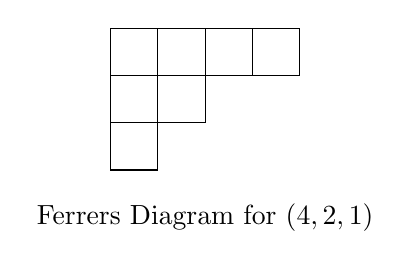
\begin{tikzpicture}[scale=0.6]
  % Ferrers diagram for (4,2,1)
  % Top row: 4 cells (\(\lambda_1=4\))
  \draw (0,0) rectangle (1,1);
  \draw (1,0) rectangle (2,1);
  \draw (2,0) rectangle (3,1);
  \draw (3,0) rectangle (4,1);
  % Second row: 2 cells (\(\lambda_2=2\))
  \draw (0,-1) rectangle (1,0);
  \draw (1,-1) rectangle (2,0);
  % Third row: 1 cell (\(\lambda_3=1\))
  \draw (0,-2) rectangle (1,-1);
  
  \node at (2,-3) {Ferrers Diagram for \((4,2,1)\)};
\end{tikzpicture}
\end{center}

Removing the leftmost column yields:

\begin{center}
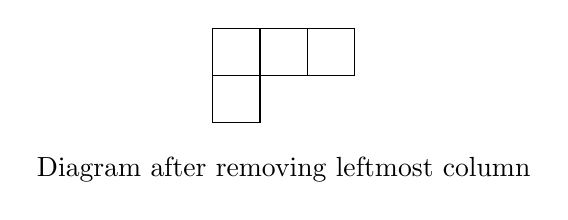
\begin{tikzpicture}[scale=0.6]
  % Diagram after removing the leftmost column from (4,2,1)
  % Top row now has 3 cells
  \draw (0,0) rectangle (1,1);
  \draw (1,0) rectangle (2,1);
  \draw (2,0) rectangle (3,1);
  % Second row now has 1 cell
  \draw (0,-1) rectangle (1,0);
  % Third row now has 0 cells (and is omitted)
  
  \node at (1.5,-2) {Diagram after removing leftmost column};
\end{tikzpicture}
\end{center}

The new diagram represents the partition \((3,1)\), which is a partition of \(7-3=4\) (since there were \(k=3\) rows, and we removed one cell per row). Note that \((3,1)\) is an element of \(P(4,\le 3)\).

\medskip

\textbf{Justification of Bijectivity.}  
The mapping
\[
\Phi\colon (\lambda_1,\lambda_2,\dots,\lambda_k) \mapsto (\lambda_1-1,\lambda_2-1,\dots,\lambda_k-1)
\]
is invertible. Given any partition \(\mu\) in \(P(n-k,\le k)\) (which has at most \(k\) parts), we can reconstruct a unique partition in \(P(n,k)\) by adding \(1\) to each part and, if necessary, appending enough parts equal to \(1\) so that the total number of parts becomes exactly \(k\). In other words, the inverse mapping \(\Phi^{-1}\) is defined by:
\[
\Phi^{-1}\colon \mu = (\mu_1,\mu_2,\dots,\mu_r) \mapsto (\mu_1+1,\mu_2+1,\dots,\mu_r+1,\underbrace{1,1,\dots,1}_{k-r \text{ times}}),
\]
with \(r\le k\). It is straightforward to check that \(\Phi\) and \(\Phi^{-1}\) are mutual inverses. Thus, the mapping \(\Phi\) is a bijection, and we have the relation:
\[
p(n,k)=|P(n,k)| = |P(n-k,\le k)| = p(n-k,\le k).
\]

\medskip

This bijective correspondence is the key step in obtaining a recursive formula for \(p(n,k)\).

\begin{corollary}
For all integers \(n\ge k\ge 1\), we have
\[
p(n,k) = p(n-k,\le k)
      = p(n-k,1) + p(n-k,2) + \cdots + p(n-k,k-1) + p(n-k,k).
\]
That is, the total number of \(k\)-partitions of \(n\) can be split into partitions of \(n-k\) with at most \(k\) parts:
\[
p(n,k) = p(n-k,\le k-1) + p(n-k,k).
\]
Moreover, since
\[
p(n-k,\le k-1)=p((n-k)+(k-1),k-1)=p(n-1,k-1),
\]
we obtain the recurrence relation
\[
p(n,k)=p(n-1,k-1)+p(n-k,k).
\]
\end{corollary}
\end{document}